% kenkyukai_template.tex を編集

%\documentstyle[epsf,twocolumn]{jarticle}       %LaTeX2.09仕様
\documentclass[twocolumn]{jarticle}
%%%%%%%%%%%%%%%%%%%%%%%%%%%%%%%%%%%%%%%%%%%%%%%%%%%%%%%%%%%%%%
%%
%%  基本 バージョン
%%
%%%%%%%%%%%%%%%%%%%%%%%%%%%%%%%%%%%%%%%%%%%%%%%%%%%%%%%%%%%%%%%%
\setlength{\topmargin}{-45pt}
%\setlength{\oddsidemargin}{0cm}
\setlength{\oddsidemargin}{-7.5mm}
%\setlength{\evensidemargin}{0cm}
\setlength{\textheight}{24.1cm}
%setlength{\textheight}{25cm}
\setlength{\textwidth}{17.4cm}
%\setlength{\textwidth}{172mm}
\setlength{\columnsep}{11mm}


%【節がかわるごとに(1.1)(1.2) …(2.1)(2.2)と数式番号をつけるとき】
%\makeatletter
%\renewcommand{\theequation}{%
%\thesection.\arabic{equation}} %\@addtoreset{equation}{section}
%\makeatother

%\renewcommand{\arraystretch}{0.95} 行間の設定

%%%%%%%%%%%%%%%%%%%%%%%%%%%%%%%%%%%%%%%%%%%%%%%%%%%%%%%%
\usepackage[dvipdfm]{graphicx}   %pLaTeX2e仕様(要\documentstyle ->\documentclass)
%%%%%%%%%%%%%%%%%%%%%%%%%%%%%%%%%%%%%%%%%%%%%%%%%%%%%%%%

% 図を別のフォルダから読み込む
\graphicspath{{./figure/}}



\begin{document}

\twocolumn[
\noindent

\hspace{1em}

情報工学実験I\hspace{-.1em}I
\hfill
\ \ B3 多田 瑞葵


\vspace{2mm}

\hrule

\begin{center}
{\Large \bf BERT を用いた深層言語処理における品詞推定の調査}
\end{center}


\hrule
\vspace{3mm}
]

\section{はじめに}
近年,人工知能や深層学習による創作に関する研究が盛んになっている.自然言語処理の分野においても小説の生成を目指した文や文章の生成などが研究されている.その一つが,生成される文の文法情報や品詞情報が正しく得られるかという課題である.文を生成する際には言葉を正しくならべる必要があり,それには正しい文法や品詞の知識と理解が欠かせない.\par
本実験では,最近注目を集めている深層言語モデルである BERT を用いて,文生成の基礎である文の品詞の情報をどの程度獲得できるのかを実験をもとに調査した.


\section{要素技術}
% 要素技術と従来手法をあわせて要素技術

  \subsection{BERT}
BERT (Bidirectional Encoder Representations from Transformers)\cite{DBLP} は,2018 年 10 月に Google の Jacob Devlin らが発表した,Transformer による双方向のエンコーダを用いた言語モデルである.BERT は入力文に対して,入力された文とその文に含まれる各単語に対応する分散表現を出力する.従来の言語モデルは特定の自然言語処理タスクにのみ対応しており,タスクに応じてモデルの修正が必要であった.しかし BERT はファインチューニングをすることで,モデルの修正をせずに様々なタスクに応用でき,汎化性に優れているという特徴を持つ.また発表当時,11 個のタスクに対して state-of-the-art を達成しており精度が高いという特徴もある.\par
BERT は事前学習モデルであり,入力文の一部の単語を “[MASK]” 記号に置き換えてその元単語を予測する「masked language model」に基づいたタスクと,2 つの入力文に対して文の連続性を識別する「next sentence prediction」のタスクによって学習してモデルを構築する.\par
本実験では,東北大学から公開されている,日本語 Wikipedia の文章を用いて事前学習されたモデル\footnote{https://www.nlp.ecei.tohoku.ac.jp/news-release/3284/}を使用した.このモデルでは,入力文を MeCab\cite{110002911717} により形態素解析し,WordPiece という手法により subword 化している.




% 脚注の入れ方
%http://www.latex-cmd.com/struct/footnote.html
% MeCab 脚注 \footnote{https://taku910.github.io/mecab/}



\section{使用データセット}
本実験では,書き言葉中心の叙述的な文を対象として品詞を推定するために毎日新聞データセット\footnote{https://www.nichigai.co.jp/sales/mainichi/mainichi-data.html}の新聞記事をデータセットとして用いた.2008 年の 1 面に掲載された記事の中から文として成立しているものを抜き出し,それぞれの文章に対して “□”,“×” などの記号,“<>” などの間に書かれた注釈等を取り除いた.
 



%\section{実験手法}
% 従来手法があるなら提案手法とする

\section{数値実験}
本実験では,文中の単語を “[MASK]” 記号に置き換えた文を入力として,“[MASK]” 記号で隠された単語の元の品詞(名詞,動詞,形容詞)を正しく推定できるかを調査した.これらは内容語と呼ばれ,文の内容を表す品詞群である.本実験ではまず文の意味を直接的に表す品詞の推定をするためにこれらの品詞から推定することにした.

  \subsection{実験の前処理}
前処理として,データセットの各文に対して分かち書きをし,単語に分割した.一文の単語の中から 1 つをランダムに選択して "[MASK]" 記号に置き換えた.名詞のデータセットでは,置き換えた箇所の元単語が名詞である文にラベル 1 を,そうでない文にラベル 0 を付与し,実験に用いるデータとした.置き換えた箇所の元単語が動詞や形容詞であるものについても名詞と同様にラベルを付与して,実験に用いるデータセットを構築した.以上の手順で名詞,動詞,形容詞の推定用のデータセットをそれぞれ 1 セットずつ用意した.\par

  \subsection{実験}
まず,データセットの各文に対して,データの偏りによる精度の差を避けるため,ラベル 0 とラベル 1 のデータ数を同じ 5000 個に揃えた.この各文を BERT に入力して,得られた各単語の分散表現を多層パーセプトロン(Multi Layer Perceptron, MLP)に入力して分類した.表 \ref{tb:1} に本実験で用いた MLP のパラメータを示す.学習率は BERT の初出論文 \cite{DBLP} で推薦されている値を使用した.BERT は最終層のみをファインチューニングしている.またデータ数が少ないため,訓練データに対して 5 分割交差検証による平均値を確認して評価した.各データセットのデータ数は,訓練データ 9000 文,テストデータ 1000 文である.



\begin{table}[t]
	\caption{実験で用いた MLP のパラメータ}
  \begin{center}
  \begin{tabular}{|c|c|} \hline
  パラメータ & 値  \\ \hline \hline
  最大入力系列長	& 256 \\ %\cline{2-2}
  隠れ層の次元数	& 768 \\
  出力層の次元数	& 2 \\
  エポック数 & 10 \\
  バッチサイズ & 10 \\
  損失関数 & Cross Entropy \\
  最適化関数 & Adam \\
  学習率 & $5\times10^{-5}$ \\ \hline
	\end{tabular}
  \end{center}
	\label{tb:1}
\end{table}




\subsection{実験結果}

図 \ref{fig:mei_acc} から図 \ref{fig:kei_loss} に,学習時の accuracy と loss の推移を示す.横軸はどちらも epoch 数を,縦軸はそれぞれ accuracy と loss を表している.表 \ref{tb:2} にテスト時の品詞の推定結果を示す.本実験はデータ数が等しい二値分類であるため,accuracy のベースラインは 0.500 である.



% \begin{minipage}{0.5\hsize} で,図を横並びに挿入できる
\begin{figure}[tbp]
      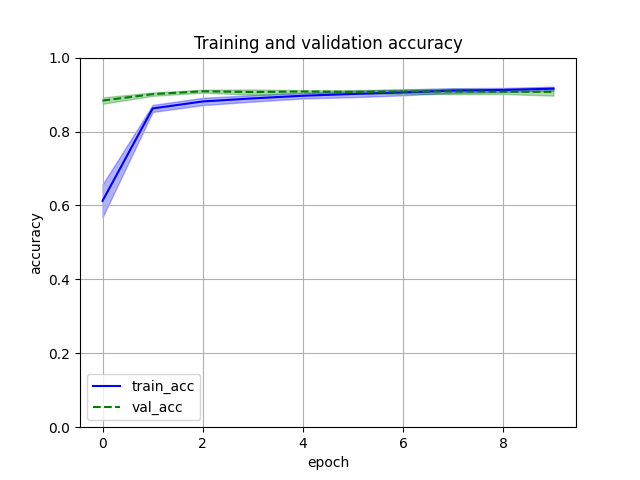
\includegraphics[width=\linewidth]{meishi_acc.png}
      \caption{名詞推定時の accuracy の推移}
      \label{fig:mei_acc}
\end{figure}
\begin{figure}[tbp]
      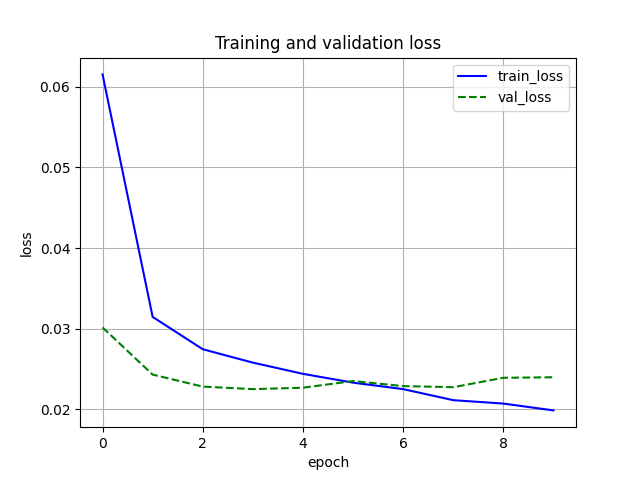
\includegraphics[width=\linewidth]{meishi_loss.png}
      \caption{名詞推定時の loss の推移}
      \label{fig:mei_loss}
\end{figure}

\begin{figure}[tbp]
      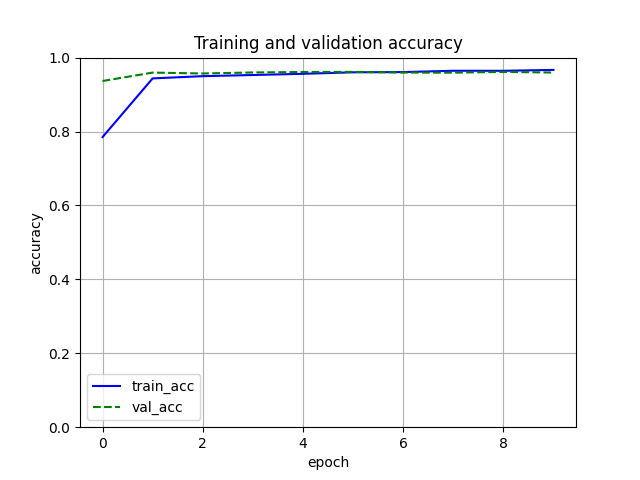
\includegraphics[width=\linewidth]{doushi_acc.png}
      \caption{動詞推定時の accuracy の推移}
      \label{fig:dou_acc}
\end{figure}
\begin{figure}[tbp]
      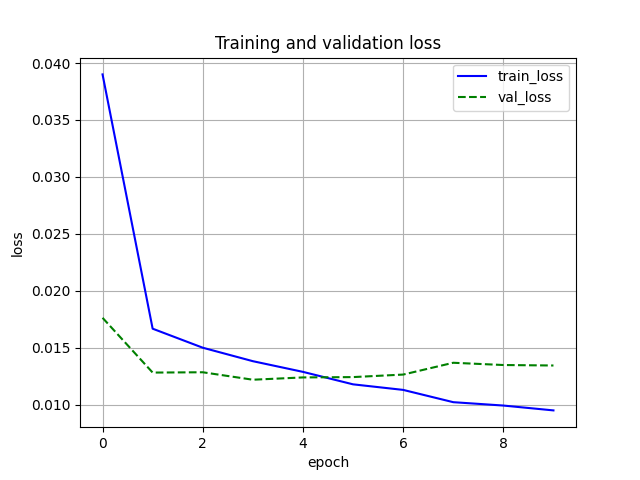
\includegraphics[width=\linewidth]{doushi_loss.png}
      \caption{動詞推定時の loss の推移}
      \label{fig:dou_loss}
\end{figure}

\begin{figure}[tbp]
      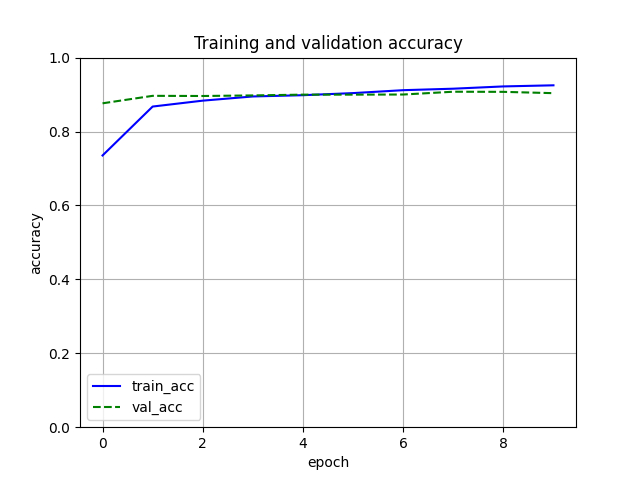
\includegraphics[width=\linewidth]{keiyoushi_acc.png}
      \caption{形容詞推定時の accuracy の推移}
      \label{fig:kei_acc}
\end{figure}
\begin{figure}[tbp]
      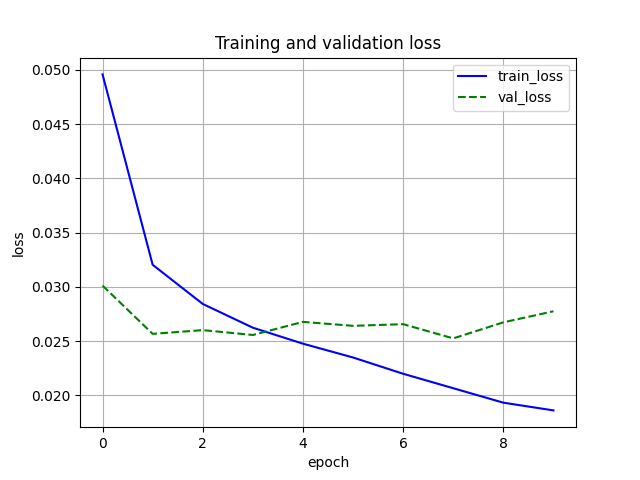
\includegraphics[width=\linewidth]{keiyoushi_loss.png}
      \caption{形容詞推定時の loss の推移}
      \label{fig:kei_loss}
\end{figure}



\begin{table}[t]
	\caption{実験精度の平均値及び標準偏差}
    \begin{center}
	\begin{tabular}{| c |  c |} \hline
  品詞 & Accuracy \\ \hline \hline
  名詞 & 0.914 (0.004) \\ %\cline{2-2}
  動詞 & 0.953 (0.004) \\
  形容詞 & 0.905 (0.004) \\
  ベースライン & 0.500 \\ \hline
	\end{tabular}
    \end{center}
	\label{tb:2}
\end{table}


 \subsection{考察}
 表 \ref{tb:2} の通り,名詞,動詞,形容詞のいずれにおいてもベースラインを大きく上回り,高い精度で品詞の推定ができた.表 \ref{tb:3} から表 \ref{tb:5} に,各品詞の推定時の出力結果の例を示す.推定を誤ったデータを確認したところ,人間の感覚でも推定しづらいものが多かった.


 \begin{table*}[t]
 	\caption{名詞の推定における出力結果の例}
     \begin{center}
 	\begin{tabular}{|c|c|p{30em}|c|} \hline
   真値 & 予測値 & 文 & [MASK] の単語 \\ \hline \hline
   0 & 0 & スエズ運河に至る紅海の入り口は、年間約2万隻[MASK]行き交う。 & が \\ \hline
   1 & 1 & このほか、[MASK]の保健衛生向上や食糧問題の解決へ日米が協力していくことで合意。 & アフリカ  \\ \hline
   0 & 1 & 免許取得前の03年3月[MASK]も無免許で車を運転し、道交法違反容疑で検挙されていた。 & に \\ \hline
   1 & 0 & 少年法は検察の再抗告を規定していないため、[MASK]13歳で刑事責任を問われなかった少年を除く4人全員の「無罪」が確定した。 & 当時  \\ \hline
 \end{tabular}
     \end{center}
 	\label{tb:3}
\end{table*}

\begin{table*}[t]
 \caption{動詞の推定における出力結果の例}
    \begin{center}
 \begin{tabular}{|c|c|p{30em}|c|} \hline
  真値 & 予測値 & 文 & [MASK] の単語 \\ \hline \hline
  0 & 0 & 最も[MASK]充足率が低かった大学は11・3\%だった。 & 定員 \\ \hline
  1 & 1 & 憲法59条の規定の多用に厳しい世論が[MASK]だ。 & 浮かん  \\ \hline
  0 & 1 & 物価が[MASK]、支援活動もあって暮らしやすい面もあるため、保護を受ける目的で市外から移住する人も少なくない。 & 安く \\ \hline
  1 & 0 & ダムの水位は2〜3メートル低下、自然に[MASK]状態になっており、決壊の危険性は低くなった。 & 流れ出る  \\ \hline
\end{tabular}
    \end{center}
 \label{tb:4}
\end{table*}

\begin{table*}[t]
 \caption{形容詞の推定における出力結果の例}
    \begin{center}
 \begin{tabular}{|c|c|p{30em}|c|} \hline
  真値 & 予測値 & 文 & [MASK] の単語 \\ \hline \hline
  0 & 0 & 結果を「見解」や「勧告」として公表、対象と[MASK]た放送局に対して内容を放送するように求める。 & なっ \\ \hline
  1 & 1 & 党幹部は「参院での採決は14日の可能性が[MASK]なってきた」と述べた。 & 高く  \\ \hline
  0 & 1 & 岩手・宮城内陸地震の被災地では19日昼からまとまった降雨が[MASK]される。 & 予想 \\ \hline
  1 & 0 &	厚労省は基本的に申請が早い方から認定作業を進めるが、原告については、一度却下されていても再申請[MASK]に諮問する。 & なし  \\ \hline
\end{tabular}
    \end{center}
 \label{tb:5}
\end{table*}



\section{まとめと今後の課題}
本実験では,文中の単語がある品詞かそうでないかの 2 クラスに分類し,BERT を用いた推定精度を確認した.結果として,名詞,動詞,形容詞のいずれにおいても,高い精度で品詞を推定できることが分かった.このことから BERT は,隠された単語であってもその単語の品詞情報を獲得することができるため,適切な品詞の単語を補って文を生成することは可能であると考えられる.\par
今後の課題としては以下のようなものが挙げられる.
\begin{itemize}
  \item 一文の複数箇所を “[MASK]” 記号に置き換えた場合にも品詞情報が正しく獲得できるかの確認
  \item 隠された単語そのものの推定
  \item 内容語以外の機能語(助詞など)を含めた推定
\end{itemize}





% 参考文献出力
\bibliography{index}
\bibliographystyle{unsrt}


\end{document}
